\documentclass[a4paper,14pt]{article}

\usepackage{comment} % Para comentar várias linhas ao mesmo tempo

%matemática
\usepackage{amsmath}
\usepackage{amssymb}

%diagramação
\usepackage{extsizes}
\everymath{\displaystyle}
\usepackage{geometry}
\usepackage{fancyhdr}
\usepackage{multicol}
\usepackage{graphicx}
\usepackage[brazil]{babel}
\usepackage[shortlabels]{enumitem}
\usepackage{cancel}
\usepackage{textcomp}
\usepackage{tcolorbox}

%tabelas
\usepackage{array} % Para melhor formatação de tabelas
\usepackage{longtable}
\usepackage{booktabs}  % Para linhas horizontais mais bonitas
\usepackage{float}   % Para usar o modificador [H]
\usepackage{caption} % Para usar legendas em tabelas
\usepackage{wrapfig} % Para usar tabelas e figuras flutuantes
\usepackage{xcolor} % Para cores do fundo de tabelas
\usepackage{colortbl} % Para cores do fundo de tabelas

%tikzpicture
\begin{comment}
	\usepackage{tikz}
	\usepackage{scalerel}
	\usepackage{pict2e}
	\usepackage{tkz-euclide}
	\usetikzlibrary{calc}
	\usetikzlibrary{patterns,arrows.meta}
	\usetikzlibrary{shadows}
	\usetikzlibrary{external}
\end{comment}


%pgfplots
\usepackage{pgfplots}
\pgfplotsset{compat=newest}
\usepgfplotslibrary{statistics}
\usepgfplotslibrary{fillbetween}

%colours
\usepackage{xcolor}



\columnsep=2cm
\hoffset=0cm
\textwidth=8cm
\setlength{\columnseprule}{.1pt}
\setlength{\columnsep}{2cm}
\renewcommand{\headrulewidth}{0pt}
\geometry{top=1in, bottom=1in, left=0.7in, right=0.5in}

\pagestyle{fancy}
\fancyhf{}
\fancyfoot[C]{\thepage}

\begin{document}
	
	\noindent\textbf{6FMA89 - Matemática} 
	
	\begin{center}Polígonos: perímetro e área (Versão estudante)
	\end{center}
	
	\noindent\textbf{Nome:} \underline{\hspace{10cm}}
	\noindent\textbf{Data:} \underline{\hspace{4cm}}
	
	%\section*{Questões de Matemática}
	
	\begin{multicols}{2}
		\noindent O perímetro de um polígono é a soma das medidas dos seus lados. A área de um polígono pode ser expressa pela quantidade de quadrados unitários necessários para preenchê-lo. \\
		\noindent\textsubscript{-----------------------------------------------------------------------}
		\begin{enumerate} 
			\item Determine o perímetro dos polígonos: \\
			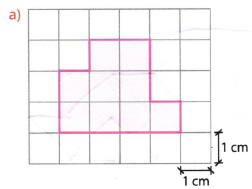
\includegraphics[width=1\linewidth]{6FMA89_imagens/imagem01} \\\\\\\\\\
			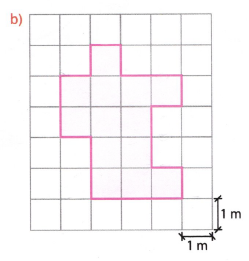
\includegraphics[width=1\linewidth]{6FMA89_imagens/imagem02}
			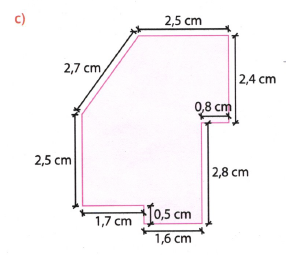
\includegraphics[width=1\linewidth]{6FMA89_imagens/imagem03}
			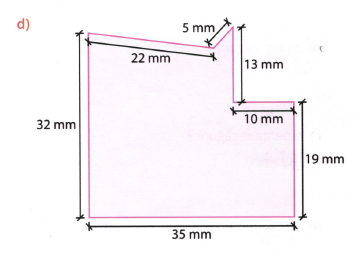
\includegraphics[width=1\linewidth]{6FMA89_imagens/imagem04}
			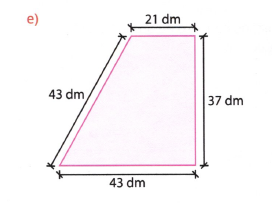
\includegraphics[width=1\linewidth]{6FMA89_imagens/imagem05}
			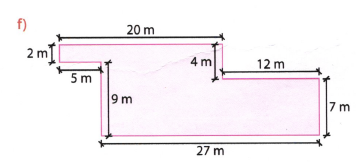
\includegraphics[width=1\linewidth]{6FMA89_imagens/imagem06}\\
			\item Na malha quadriculada dos itens a seguir, cada quadrado tem 1 cm² de área. Determine a área dos polígonos. \\
			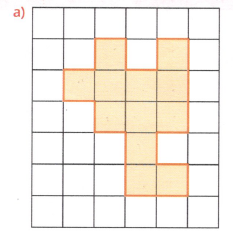
\includegraphics[width=1\linewidth]{6FMA89_imagens/imagem07}
			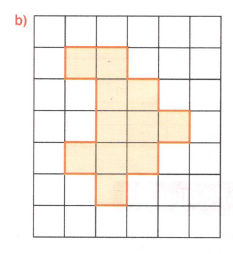
\includegraphics[width=1\linewidth]{6FMA89_imagens/imagem08}
			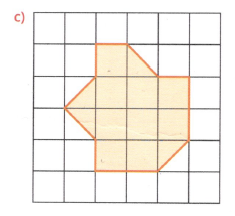
\includegraphics[width=1\linewidth]{6FMA89_imagens/imagem09}
			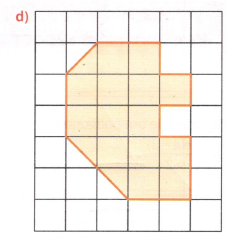
\includegraphics[width=1\linewidth]{6FMA89_imagens/imagem10}
			\item A área externa de uma casa em destaque na figura deverá ser pavimentada e cercada por um muro. Considere a malha cujos quadrados de 1 m $\times$ 1 m têm área igual a 1 m². \\
			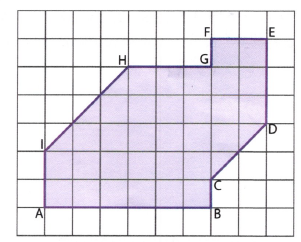
\includegraphics[width=1\linewidth]{6FMA89_imagens/imagem11}
			\begin{enumerate}[a)]
				\item Qual é o perímetro da área externa se $CD = 3$m e $HI = 4$m? \\\\\\\\\\\\\\\\
				\item Sabendo que não haverá muro em $AB$ e que o muro em $AB$ e que o muro de 1,5 m de altura custa 15 reais por metro construído, determine o custo desse muro. \\\\\\
				\item Qual é a área a ser pavimentada? \\\\\\
				\item Quanto será gasto na pavimentação da área externa, ao custo de 6 reais por metro quadrado? \\\\\\
			\end{enumerate}
			%61 a 63
			\item Calcule o perímetro de cada polígono abaixo. \\
			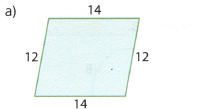
\includegraphics[width=1\linewidth]{6FMA89_imagens/imagem12}
			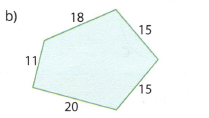
\includegraphics[width=1\linewidth]{6FMA89_imagens/imagem13}
			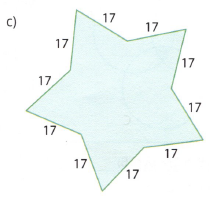
\includegraphics[width=1\linewidth]{6FMA89_imagens/imagem14}
			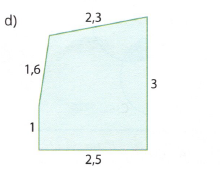
\includegraphics[width=1\linewidth]{6FMA89_imagens/imagem15}
			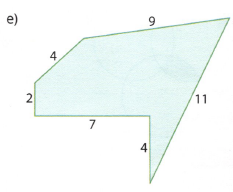
\includegraphics[width=1\linewidth]{6FMA89_imagens/imagem16} \newpage
			\item No quadrilátero abaixo, o valor de $a$ é 3. Neste caso, o perímetro desse polígono é: \\
			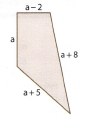
\includegraphics[width=0.5\linewidth]{6FMA89_imagens/imagem17}
			\begin{enumerate}[a)]
				\item 20
				\item 21
				\item 22
				\item 23
				\item 24
			\end{enumerate}
			\item O Sr. Alvarez pretende reformar sua casa e escolheu placas de cerâmica para serem colocadas nos pisos da área de serviço e da cozinha, como mostra a figura: \\
			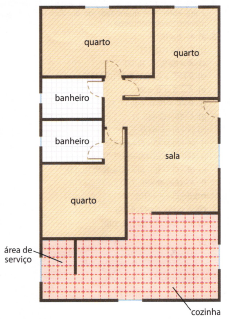
\includegraphics[width=1\linewidth]{6FMA89_imagens/imagem18} \\
			Considerando que cada placa de cerâmica é um quadrado de área 0,04 m², responda: \\
			\begin{enumerate}[a)]
				\item Qual é a área, em m², a ser coberta pelas placas de cerâmica? \\\\\\\\\\\\
				\item Se cada placa custa R\$ 12,00, qual será o gasto do Sr. Alvarez com esse piso? \\\\\\\\\\\\
			\end{enumerate}
		\end{enumerate}
		$~$ \\ $~$ \\ $~$ \\ 
	\end{multicols}
\end{document}